\documentclass[12pt]{article}
\usepackage[letterpaper, margin=1in]{geometry}
\usepackage{graphicx}
\usepackage{subcaption}
\graphicspath{{./Figures/}}
\usepackage{hyperref}
\usepackage{parskip}
\usepackage{amsmath}
\usepackage[framed, numbered]{matlab-prettifier}
\lstset{inputpath=../}
\usepackage{titlesec}
\usepackage{gensymb}

\titleformat*{\section}{\large\bfseries}
%\allowdisplaybreaks

% remove vertical spacing above top figure
\makeatletter
\setlength{\@fptop}{0pt}
\makeatother
%

\title{ELECENG 3CL4 Lab 4 Report}
\author{
    Aaron Pinto \\
    pintoa9 \\
    L02
    \and
    Raeed Hassan \\
    hassam41 \\
    L02
}

\begin{document}

\maketitle
\clearpage

\section*{Member Contributions} % copied from lab doc
Both group members contributed an even amount to both the exercises and the report. Both members went through the exercises together and contributed to all sections of the report.

\section*{Objective} % objective
To use the root locus technique to design a phase lead compensator for a marginally-stable servomotor.

\setcounter{section}{1}
\section{Design of Phase-Lead Compensator}
The procedure that was applied to design a phase lead compensator with desired design requirements was the same procedure followed in the pre-lab exercises.

The phase lead compensator was designed in a MATLAB script, with the code relevant to the design of the compensator found in Listing~\ref{listing:design_p1}. The procedure is detailed in comments found in the MATLAB script. The parameters of the desired phase lead compensator were found to be $z = 8$, $p = 20.7149$, and $k_c = 1.8154$. The resulting phase lead compensator controller $G_c(s) = 1.8154 \frac{s + 8}{s + 20.7149}$. 

\lstinputlisting[style=Matlab-editor, caption={Design of phase lead compensator}, label={listing:design_p1}, firstline=1, lastline=49, firstnumber=1]{lab4_calc.m}

The velocity error constant is found using the MATLAB code in Listing~\ref{listing:design_p2}. The velocity error constant was found to be 19.6943.

\lstinputlisting[style=Matlab-editor, caption={Velcoity error constant computation}, label={listing:design_p2}, firstline=51, lastline=52, firstnumber=51]{lab4_calc.m}

The transfer function for the closed-loop system was generated in Listing~\ref{listing:design_p3}. The transfer function $T_s = \frac{354.1s + 2833}{s^3 + 27.66s^2 + 498s + 2833}$. The poles of the transfer function were placed at $-9.6115 \pm 15.6025j$ and $-8.4364$, and the zero of the transfer function was placed at $-8$.

\lstinputlisting[style=Matlab-editor, caption={Transfer function computation}, label={listing:design_p3}, firstline=54, lastline=61, firstnumber=54]{lab4_calc.m}

The step response is plotted using the MATLAB code shown in Listing~\ref{listing:design_p4}. The plot of the step response is shown in Figure~\ref{fig:step_response}.

\lstinputlisting[style=Matlab-editor, caption={Step response}, label={listing:design_p4}, firstline=63, lastline=65, firstnumber=63]{lab4_calc.m}

The unit ramp response is plotted using the MATLAB code shown in Listing~\ref{listing:design_p5}. The plot of the unit ramp response is shown in Figure~\ref{fig:unit_ramp_response}.

\lstinputlisting[style=Matlab-editor, caption={Unit ramp response}, label={listing:design_p5}, firstline=68, lastline=71, firstnumber=68]{lab4_calc.m}

\begin{figure}[h!]
	\centering
	\begin{subfigure}[b]{0.47\textwidth}
		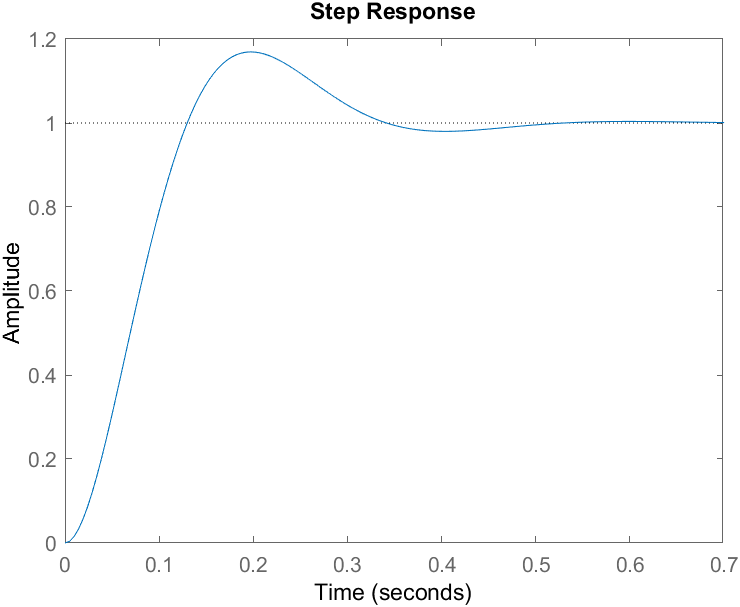
\includegraphics[width=\textwidth]{step_response}
		\caption{\label{fig:step_response}Step Response}
	\end{subfigure}
	\begin{subfigure}[b]{0.47\textwidth}
		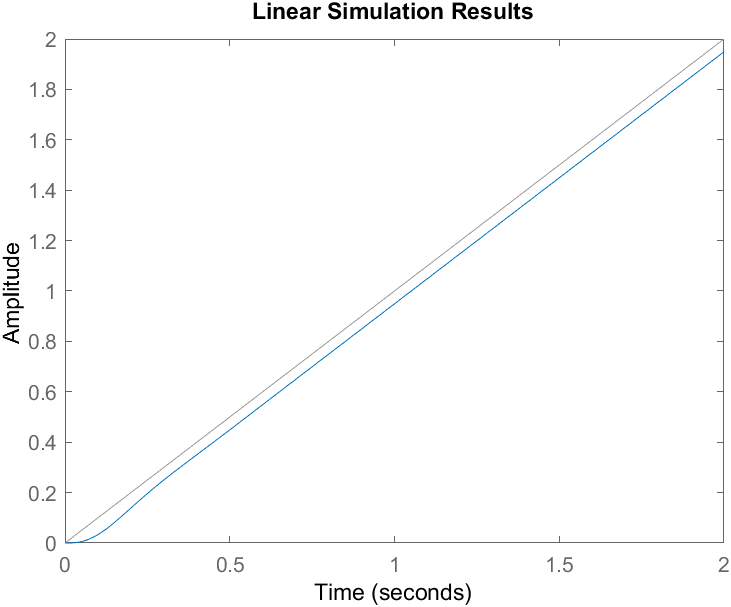
\includegraphics[width=\textwidth]{unit_ramp_response}
		\caption{\label{fig:unit_ramp_response}Unit Ramp Response}
	\end{subfigure}
	\caption{Responses of Closed-Loop Transfer Function $T(s)$}
\end{figure}

We can see from the step response in Figure~\ref{fig:step_response} that we are close to our desired design requirements. The percent overshoot is slightly less than 20\% at around 17\%, and the settling time is around the 0.5 sec requirement. The steady-state error for the unit ramp response in Figure~\ref{fig:unit_ramp_response} is around $0.05$, which matches the calculated steady-state error value for the unit ramp response (1 / velocity error constant = 0.0508). 

As our design was done using approximations for a second-order system with no zeros, it is expected that there will be some discrepancies in the results as the system in use for the servomotor is a third-order system with one zero. However, we can see that the approximations still allow us to design a system that is close to meeting the design requirements. Such a system could be a good initial design that could later be adjusted to get closer to the design requirements.

\section{Experiment with Phase Lead Compensator}
The design was simulated in MATLAB and Quanser with the servomotor model. The amplitude of the disturbance was set to 0. The numerator coefficients of the controller were $k_c$ $(1.8154)$ for s term and $k_cz$ $(1.8154 \cdot 8)$ for the constant term, and for the denominator they were 1 for the s term and $p$ $(20.7149)$ for the constant term. We entered them into the controller block in descending order of power.

The step response was checked with a square wave at the input. The measured peak overshoot and 2\% settling time were 5.08\% and approximately 0.3 seconds, respectively. These values are both below our target desired requirements and much further away than we were expecting from our design. The step response in simulation can be seen in Figure~\ref{fig:exp2_step}.

\begin{figure}[h!]
	\centering
	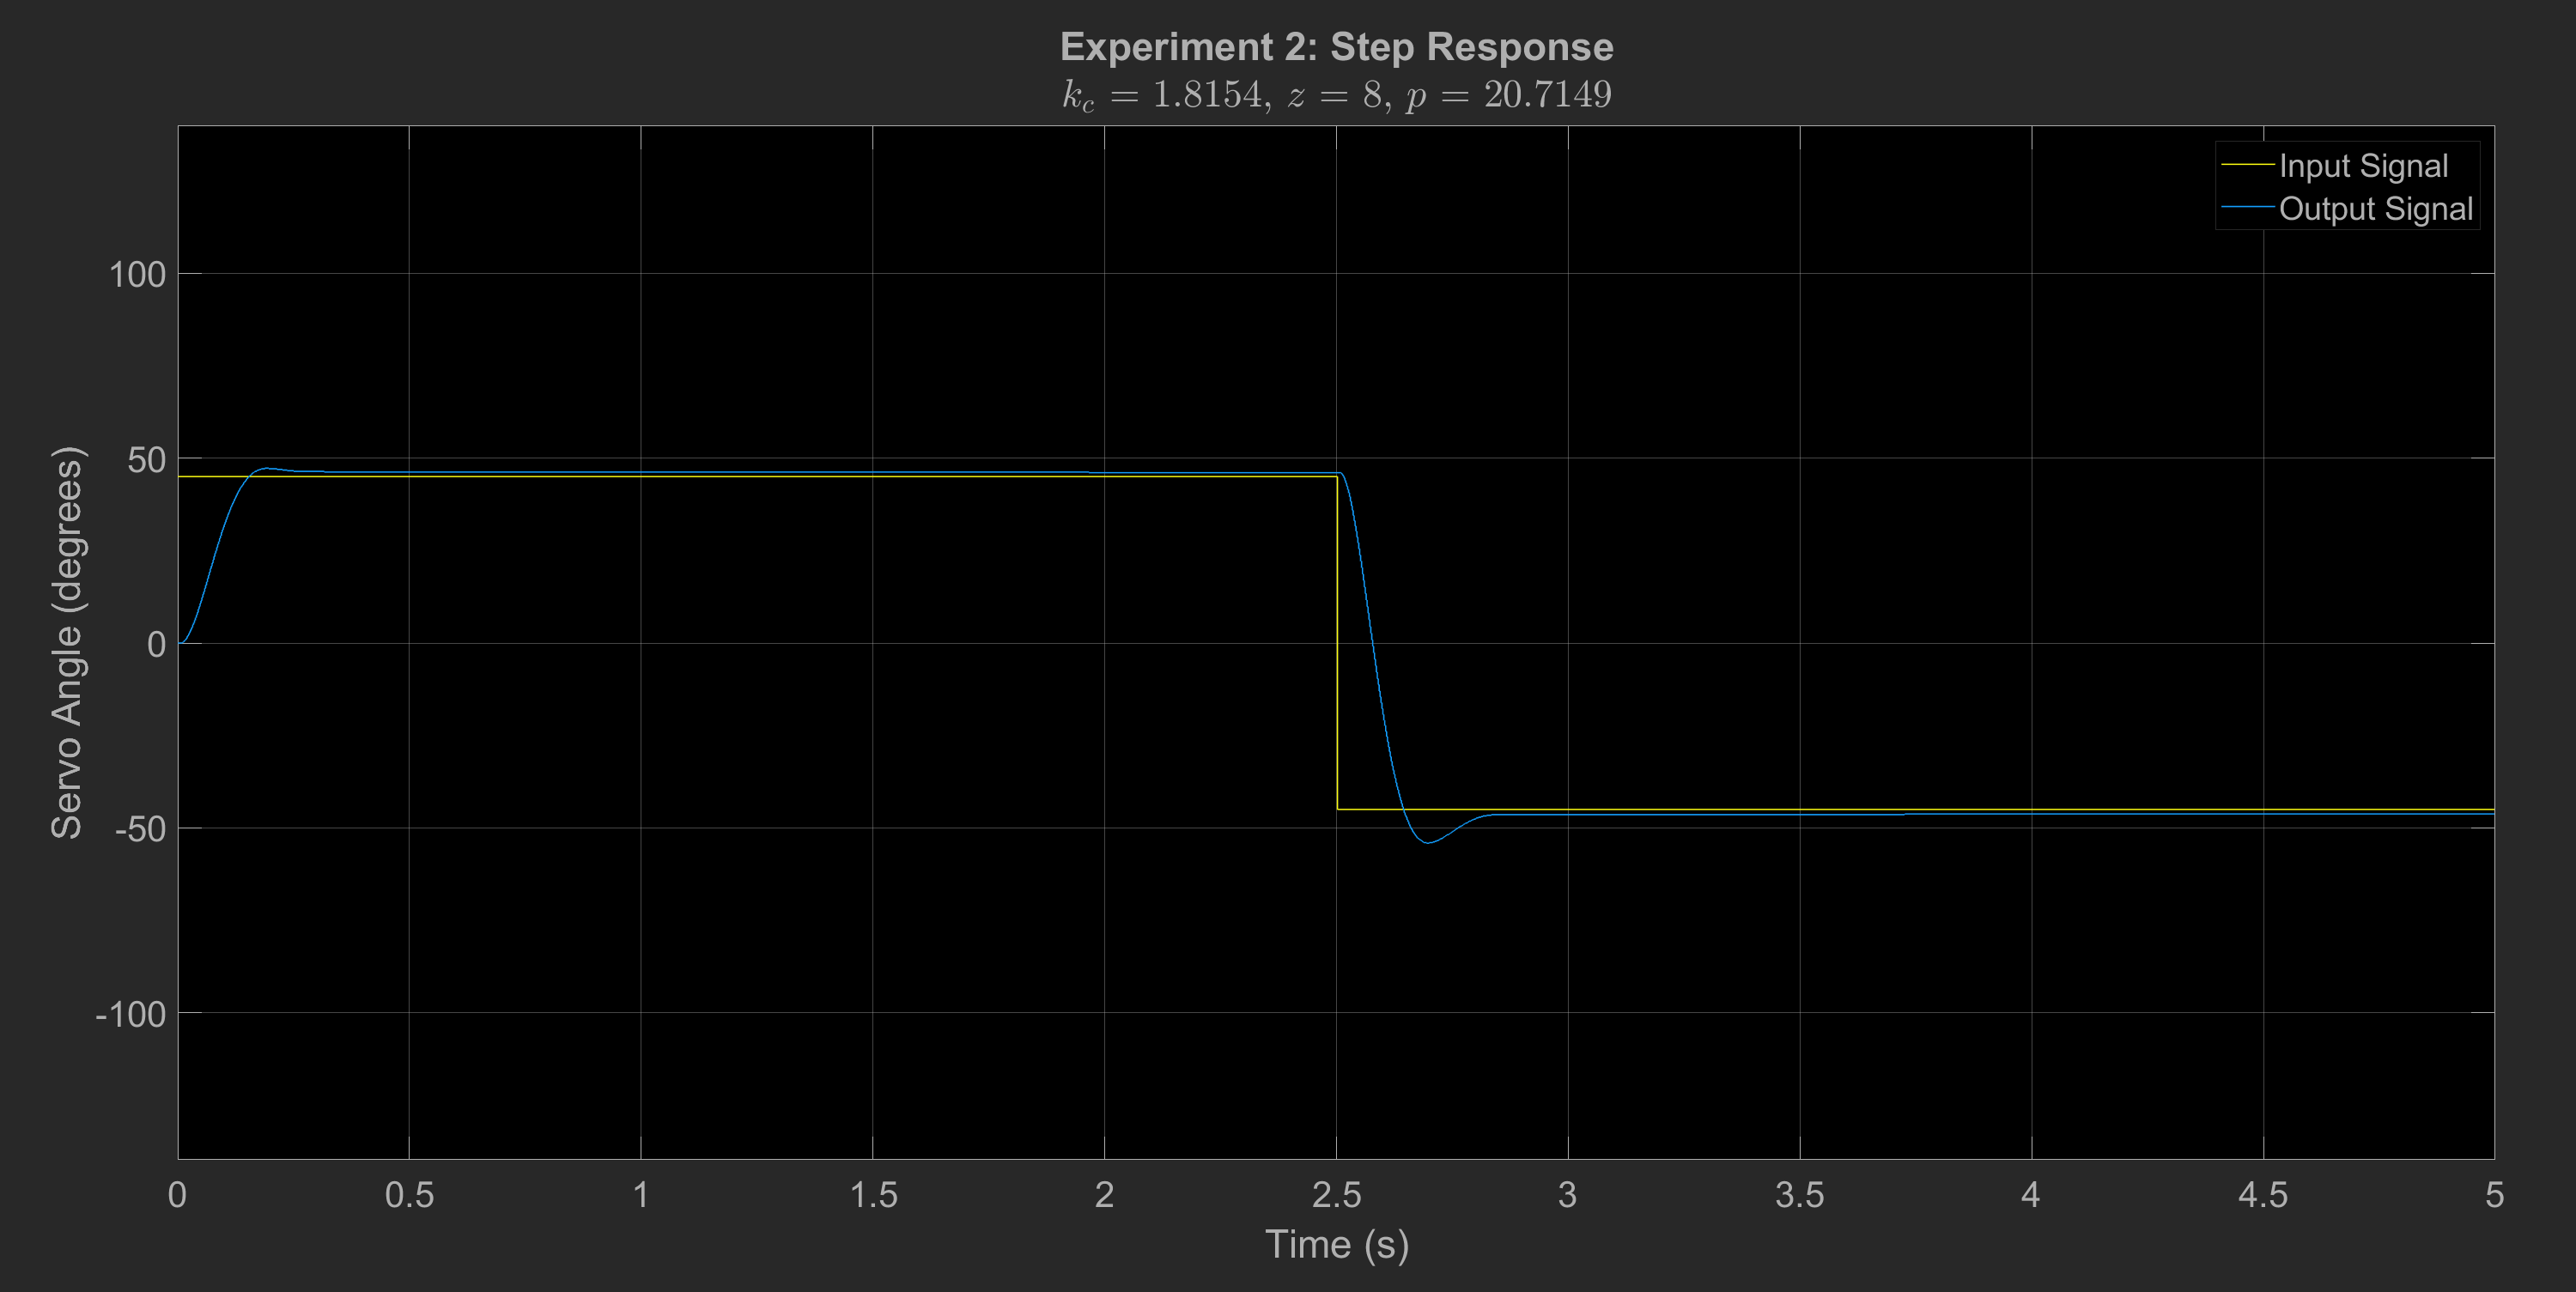
\includegraphics[width=\textwidth]{exp2_step_response}
	\caption{\label{fig:exp2_step}The Step Response of the Design in Simulation}
\end{figure}

The unit ramp response was checked with a triangular wave at the input. The measured steady state error was $7.94\degree$, or 0.1386 radians. This is much greater than the calculated 0.0508 radians for the design. The unit ramp response in simulation can be seen in Figure~\ref{fig:exp2_unit_ramp}.

\begin{figure}[h!]
	\centering
	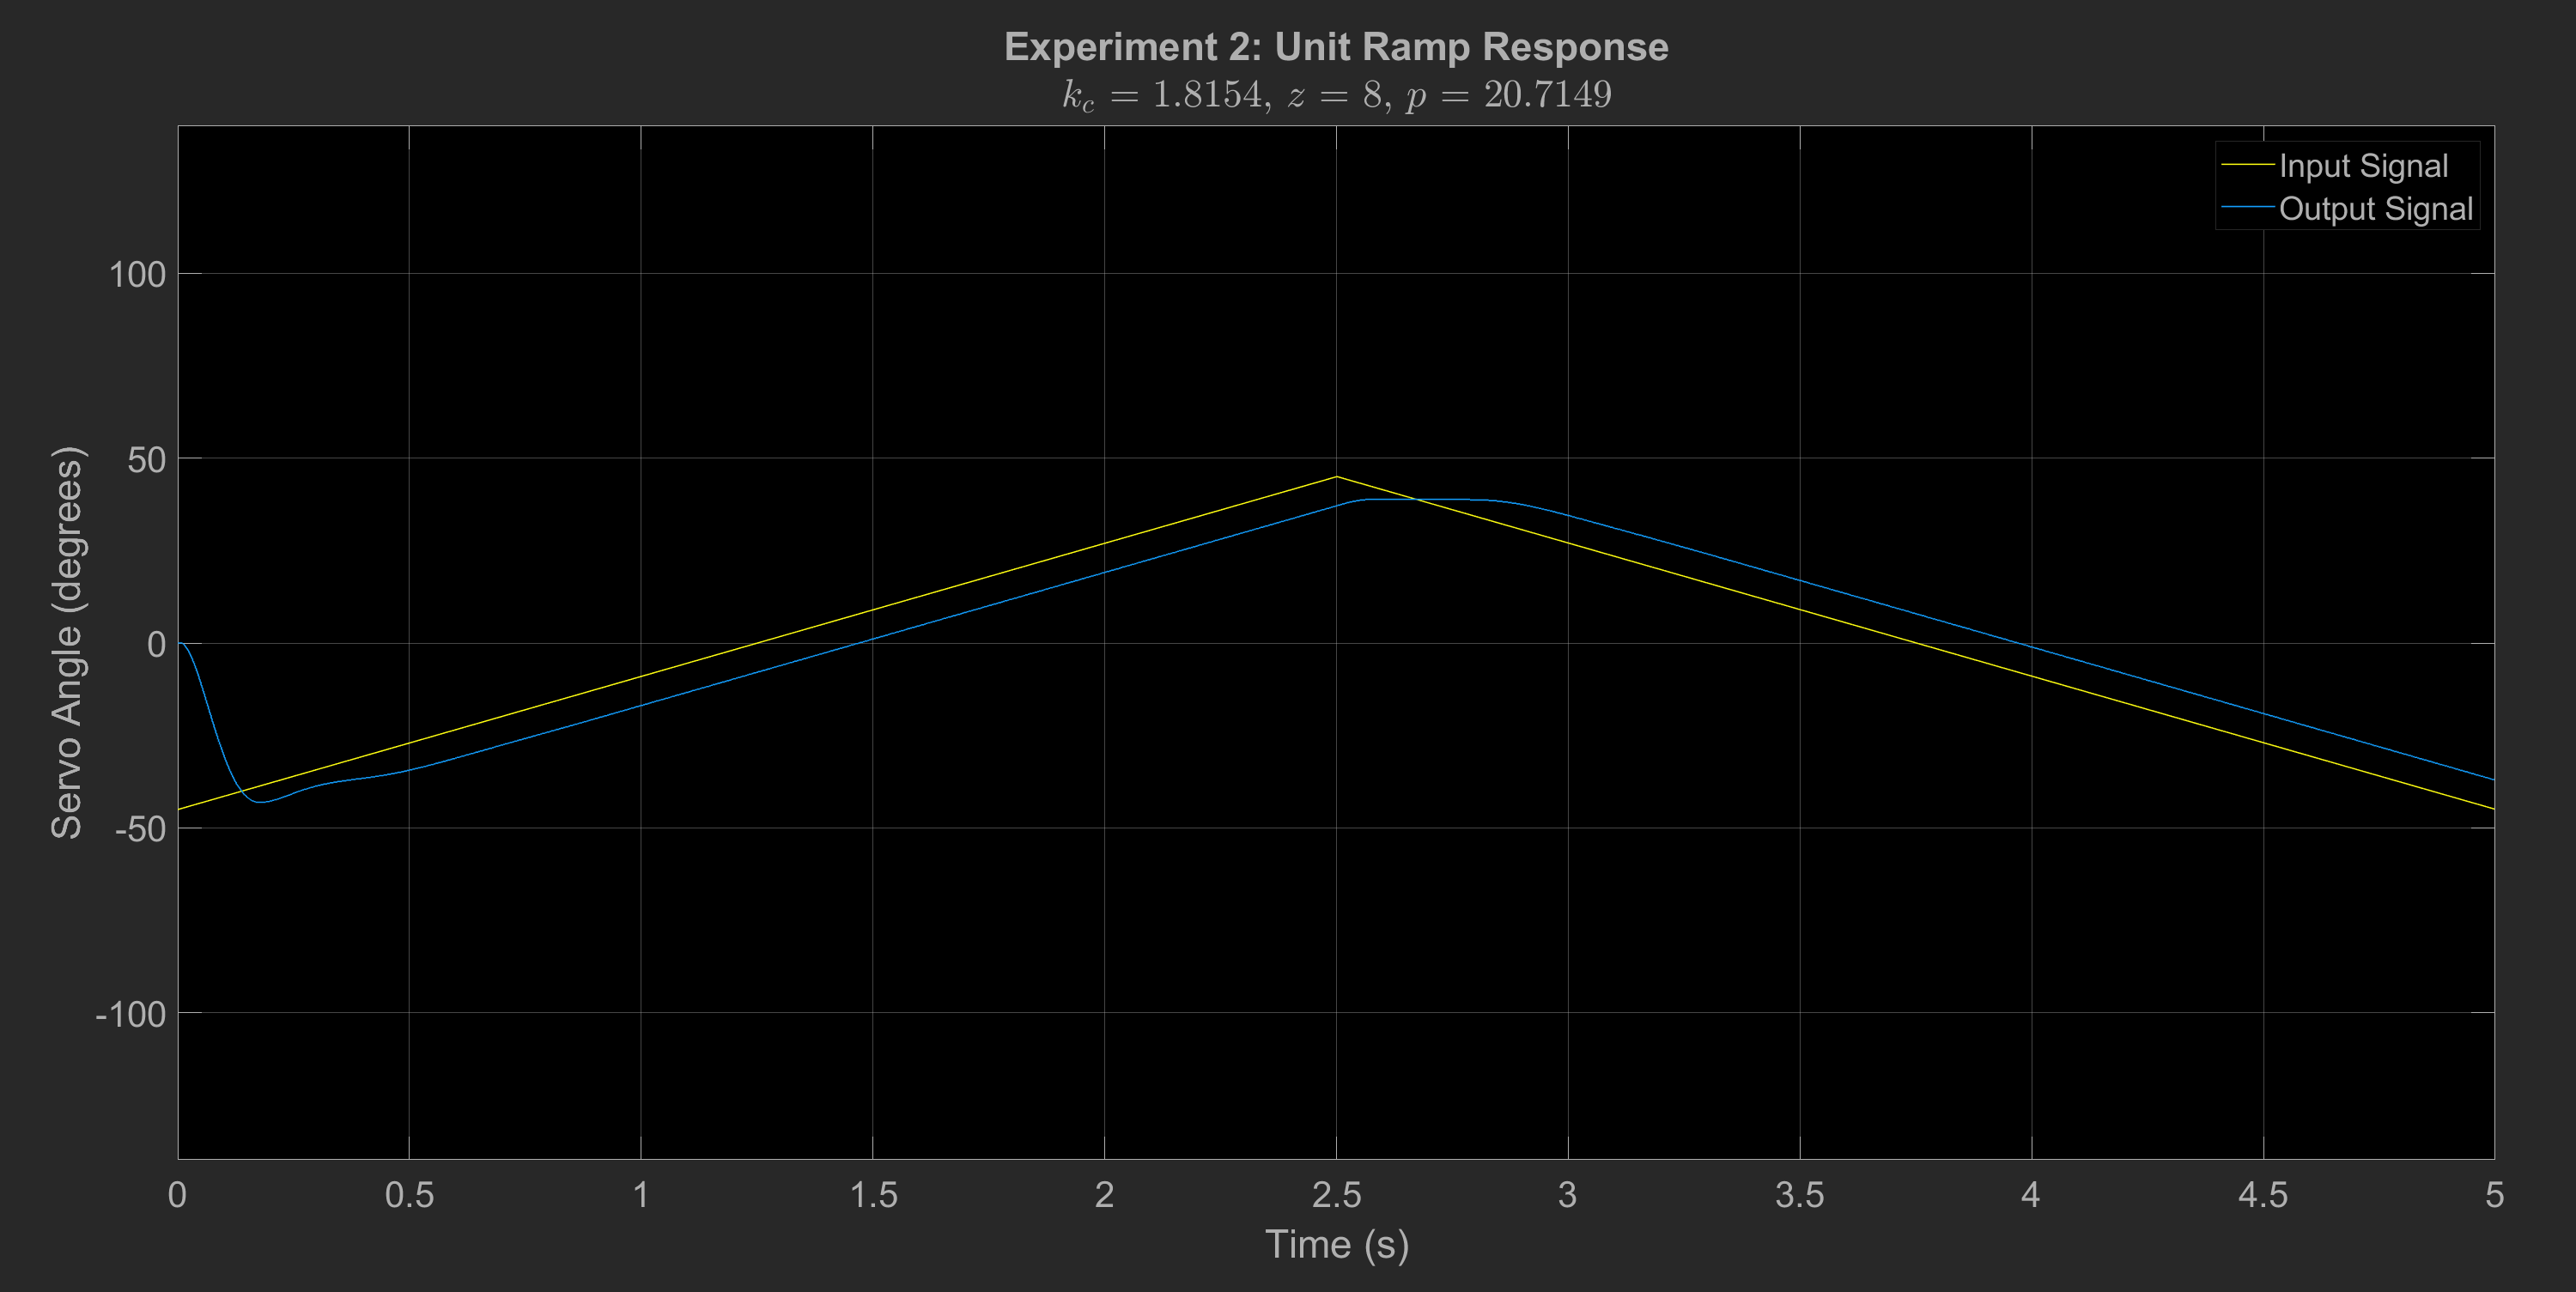
\includegraphics[width=\textwidth]{exp2_unit_ramp_response}
	\caption{\label{fig:exp2_unit_ramp}The Unit Ramp Response of the Design in Simulation}
\end{figure}

% exp2, reasons that contribute to the deviation (non-linearities, order of model)
Both the step response and unit response had significant deviation from the expected results. While our calculations were based on approximations for a second-order system with no zeros, the are significant differences between the step response (Figure~\ref{fig:step_response}) and unit ramp response (Figure~\ref{fig:unit_ramp_response}) from the design which was verified in Experiment 1, and the simulation model in this experiment.

Potential source of the discrepancies could be the inherent non-linear effects of the simulation model, or model mismatch between the simulation model and the design model. It is also possible that the values of $A$ and $\tau_m$ calculated in Lab 2 are incorrect, causing discrepancies between our design model and the simulation model.

\end{document}
